\documentclass{article}

\author{Nicol\'o Ruggeri}
\title{Combinatorial Optimization Final Report}
\date{\null}

\usepackage{amsmath}
\usepackage{amsfonts}
\usepackage{hyperref}
\hypersetup{
     colorlinks = true,
     linkcolor = blue,
     anchorcolor = blue,
     citecolor = blue,
     filecolor = blue,
     urlcolor = blue
     }
     
\usepackage{graphicx}


\begin{document}
\maketitle

\section{Introduction and  First Notations}
In this report we analyze the performances of two different methods for solving a particular instance of the TSP problem. Specifically, we solve the problem presented below with a linear programming network flow formulation, as requested in homework 1, and with a genetic algorithm presented in section \ref{sec:algorithm}. \\
In our case we formulate the problem on a complete graph $G = (V, E)$ where the adjacency matrix $A \in \mathbb{R}^{|V|}$ of $G$ is symmetric and dense. In our case we consider a weighted graph, so that $a_{i,j} \in \mathbb{R}_{\ge 0}$ is the cost of moving from point $j$ to $i$. We will explain how these distances are generated in section \ref{sec:data}.\\
The particular properties of the matrix reflect two assumptions that we make on our model, namely:
\begin{itemize}
\item $A$ symmetric. This means that the cost of going from $j$ to $i$ is the same as going the other way around. This makes sense for the underlying practical problem at hand, i.e. the one of a drill moving from position $i$ to $j$
\item $A$ dense (and in the particular case of our experiments, with almost all elements strictly positive, see sections \ref{sec:data} and \ref{sec:experiments}). With a slight abuse of terminology, here we mean that all entries of $A$ are available (or, equivalently for the problem, lesser than infinite). This reflects the fact that $ij \in E \hspace{2mm} \forall i, j$, i.e. the drill can move between any two arbitrary points
\end{itemize}
In the following section we will refer to points equivalently as nodes, and to the connections between them as edges (from the graph formulation).


\section{Data Generation}\label{sec:data}
\subsection{Distance Matrix}
We frame the problem as that of moving between points in the unitary square $[0, 1]^2$. Notice that this doesn't represent a restriction, since it can be seen as a rescaling of a problem of any size. Given that we have a finite number of points, we can number them from $1$ to $n$, so that the vertex set of the graph is $V = \{ 1, \ldots, n  \}$. Now we consider these two dimensional sampled vectors $x_i \in [0, 1]^2 $, that represent the position of every point in the drilling board. If we want to generate the cost matrix $A$ from these points, a natural interpretation could be to assume a movement time proportional to the distance between the points. In fact in the experiments section \ref{sec:experiments} we consider a distance matrix given by
\begin{equation}\label{eq:cost}
a_{ij} := {|| x_i - x_j ||}_2
\end{equation} 
The choice of the 2-norm is arbitrary, and could be replaced by any euclidean norm, which could in principle affect the final optimal solution. \\
Notice that this approach is easily generalized in many ways. For example to exclude some edges from the final solution we just need to impose $a_{ij} = +\infty$. To differenciate the cost between points we can substitute the formulation above with $a_{ij} = f(x_i, x_j)$ for some function $f$ (that doesn't even need to be symmetric in the arguments, as the genetic algorithm from section ).  

\subsection{Experimental Data}\label{sec:experimental_data}
Following the process above, we just need to generate any number $n$ of points $x_i \in [0, 1]^2 $, and then build the cost matrix that we will input to the solvers. In our case we decided to generate these points at random in the following way:
\begin{itemize}
\item a number $n_1$ of points is generated according to a mixture of equiprobable two-dimensional gaussians with given variance $\sigma^2$ and means $\mu_1, \ldots, \mu_k$. Since the sampled points could end up being outside the allowed space, we clip all the points' coordinates in $[0, 1]$. 
\item the remaining $n-n_1$ points are radomly distributed on a fixed granularity grid on  $[0, 1]^2$. This allows to have some clusters, given by the gaussians, and some other points scattered on the square. 
\end{itemize}
Notice that this procedure allows, with small probability, overlapping points. This is not a problem for our model, as the solvers need to be able to recognize this peculiarity and find a solution where such points are visited sequentially, since this movement has cost 0 according to equation \eqref{eq:cost}.


\section{The Genetic Algorithm}\label{sec:algorithm}
After the use of the OPL model for homework 1, we decided to implement a heuristic for the solution of the problem described above in homework 2. Specifically, we designed a genetic algorithm, represented as a class \textit{TSPSolver} in the code attached to this report. Moreover, we decided to implement this class from scratch. This choice is not due to the lack of Python libraries for genetic algorithms (see for example \href{https://deap.readthedocs.io/en/master/}{DEAP} or  \href{https://pyeasyga.readthedocs.io/en/latest/index.html}{pyeasyga}), but rather to a will to better understand the challenges of a complete implementation of a model, aa well as to a undoubtedly enhanced learning experience. \\
Details about the implementation are included in the following section.

\subsection{Implementation Details}
The genetic algorithm represents solutions to the TSP problem using the path representation. This means that a solution is a permutation of $\{0, \ldots, n-1\}$ where the nodes are listed in order of visit. The only neighbourhood considered is the standard 2-opt neighbourhood. \\
The following options have been made available in the implementation (see attached for further details, it has been made as clear and documented as possible):
\begin{itemize}
\item \textbf{initialization}: individuals (i.e. solutions) are initialized at random. Every generation is made up of a customized size of individuals. At initialization time it is possible to choose a fraction of individuals to substitute with their best 2-opt neighbour

\item \textbf{selection of individuals}: all selection types seen in class have been made available, namely montecarlo, linear ranking and $n$-tournament. This selection type affects which individuals are chosen for mating.

\item \textbf{mating}: two types of mating have been made available. The first is the selection of a given number of pairs of individuals. Every pair gives rise, according to the type of crossover, to one of two individuals as offspring. The second is the selection of a "mating pool": a number of individuals is chosen, and every possible couple undergoes crossover.

\item \textbf{crossover}: many types of crossover are available in literature, two possible reviews are \cite{gupta2011study} and \cite{abdoun2012comparative}. Since we found more clarity in the explanations from \cite{gupta2011study}, we implemented all the crossover types presented there. For clarity, we stick to the notation in reference in the code (which is also pretty intuitive, see the private method \textit{TSPSolver.\_crossover})

\item \textbf{mutation}: with a customized probability, every new individual undergoes mutation. If mutated, every individual is substitued with a random 2-opt neighbour

\item \textbf{generation replacement}: it is possible to keep the best $m$ individuals among the old and new generation, or to remove the worst $m$

\item \textbf{stopping criterion}: there are some stopping criteria available: the maximum number of non improving evolution steps, the time limit, the target score (i.e. stop as soon as the best individual passes a certain score threshold) and the maximum number of generations. These can also be used in combination.

\item \textbf{fitness function}: here we allowed no option but the total cost of the path (including the return to the initial node 0). This point is just to highlight that for efficiency recursive evaluation of the fitness score has been used when possible (i.e for all points from the second generation onward)
\end{itemize}
As a final remark, we would like to to underline that the code has been factorized as much as possible, building appropriate private (or public, even though the difference is almost non-existent in Python) methods for \textit{TSPSolver}. This allows modification/integration of everyone of these customizations with relative ease. The code is also available on \href{https://github.com/NRuggeriProjects/Combinatorial-Optimization}{GitHub}.

\subsection{Implementation Challenges}
One of the main reasons for the usage of genetic algorithms is their relative speed and ease of implementation. We found that this is actually true, with just some caveats. While the implementation of the single parts of the algorithm is not very challenging, especially due to the fact that the procedure is well organized into distinct sections (selection, mating, crossover, etc.) and due to the (in this case) very clear and explicative metaphor with population evolution. One downside, though, is that in the moment in which one wants to allow more options, things could get messy. For this reason we report, as main difficulty encountered, the need to keep every functionality properly organized, mainly by a great deal of code factorization. As we said above, this need has in the end made the code more tidy and organized, with the possibility to add new features with relative ease.




\section{Experiments}\label{sec:experiments}
As requested for the homework, here we present a comparison of the performances of the exact OPL solver, with the network flow formulation, and the genetic algorithm. The datasets are built as follows: following the procedure from section \ref{sec:experimental_data}, we produce three datasets of sizes 20, 100 and 200 nodes. In these, half of the points come from the gaussian mixture, the other half are scattered on a grid. Plots of the data are presented in figure \ref{fig:datasets}.

\begin{figure}
    \centering
    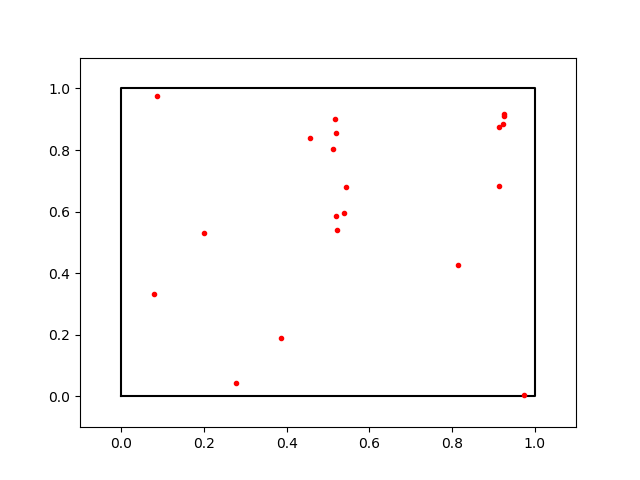
\includegraphics[width=0.3\textwidth]{pics/experimental_data_20.png}
   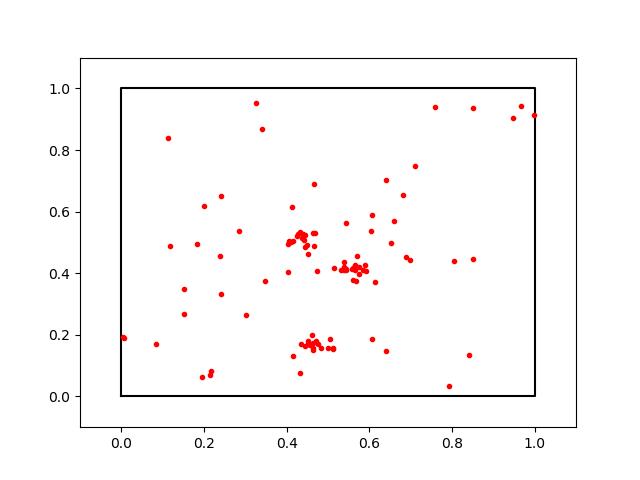
\includegraphics[width=0.3\textwidth]{pics/experimental_data_100.png} 
   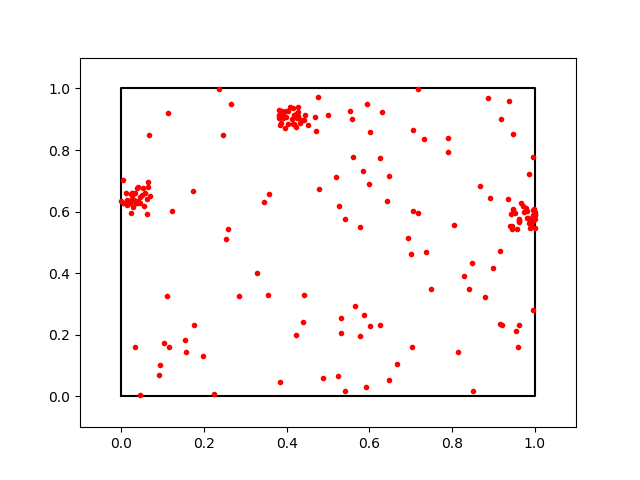
\includegraphics[width=0.3\textwidth]{pics/experimental_data_200.png}
    \caption{synthetic datasets used for the experiments. The sizes are respectively of 20, 100 and 200 nodes. Gaussian clusters points are visible among all other points.}
    \label{fig:datasets}
\end{figure}

For evaluation, we run the exact solver and the genetic algorithm 5 times each on each of the first two datasets. We just run once on the third one, allowing a longer time limit. This procedure is justified by the fact that the variability in the results from the first two datasets is so low that it is effectively approximated by zero. CHECK THIS ALSO FOR GENETIC ALGORITHM, AND DECIDE IF TO INCLUDE THE VARIANCE FOR GENETIC ALGORITHM. We comment the results separately in the following sections.

\paragraph*{20 nodes dataset}
INCLUDE IMAGE ASAP.
The genetic algorithm solver has been trained using the following parameters: \\
\newline
\textit{TSPSolver(
        init\_size=100, init\_type='best2opt', init\_best2opt\_frac=0.2, fitness='total\_cost',
        selection='montecarlo', mating='tuples', mating\_n=100, crossover='OX', mutation\_prob=0.2,
        gen\_replacement='keep\_best', gen\_replacement\_par=100,
        stopping=\{'time': 1000, 'not\_improving\_gen': 1000\}
    )} \\
\newline
where the important points are: the use of a random $0.2$ best-2opt improvement at initialization, initial population 100 individuals, 100 matings at every generation, $0.2$ probability of mutation and fixed population size of the 100 best elements (see documentation or help from \textit{TSPSolver.\_\_init\_\_}). \\
For this small instance the exact solution is reached in a short time from the OPL solver. It is interesting to see that also the genetic algorithm succedes in finding the optimal solution in the majority of the instances. 
ADD PART ABOUT PLOT COMMENT AND PLOT

\paragraph*{100 nodes dataset}
The genetic algorithm solver has been trained using the following parameters: \\
\newline
\textit{TSPSolver(
        init\_size=1000, init\_type='best2opt', init\_best2opt\_frac=0.2, fitness='total\_cost',
        selection='montecarlo', mating='tuples', mating\_n=1000, crossover='OX', mutation\_prob=0.2,
        gen\_replacement='keep\_best', gen\_replacement\_par=1000,
        stopping={'time': 1000, 'not\_improving\_gen': $+\infty$}
    )} \\
\newline
To allow for a fair comparison between the two methods, the same time constraint of 1000 seconds has been applied. As we can see, the size of the population, both at initialization and during evolution, has been increased to comply with the bigger problem size.


\paragraph*{200 nodes dataset}
The genetic algorithm solver has been trained using the following parameters: \\
\newline
\textit{TSPSolver(
    init\_size=2000, init\_type='best2opt', init\_best2opt\_frac=0.2, fitness='total\_cost',
    selection='montecarlo', mating='tuples', mating\_n=2000, crossover='OX', mutation\_prob=0.2,
    gen\_replacement='keep\_best', gen\_replacement\_par=2000,
    stopping={'time': 10000, 'not\_improving\_gen': $+\infty$}
)} \\
\newline
Again, both methods have been restricted with the same stopping criterion, in this case 10000 seconds of solution time.


\null \newline
As a final remark, we maybe need to highlight the fact that the genetic algorithm has not undergone extensive parameter optimization, both for reasons of time and because results were satisfying using "reasonable" choices. However, with more time also bayesian optimization techniques can be applied ADD REFERENCEEEEEEEE




\newpage
\bibliographystyle{ieeetr}
\bibliography{bibliography}
\end{document}